\subsection{坐标重置}
\begin{center}

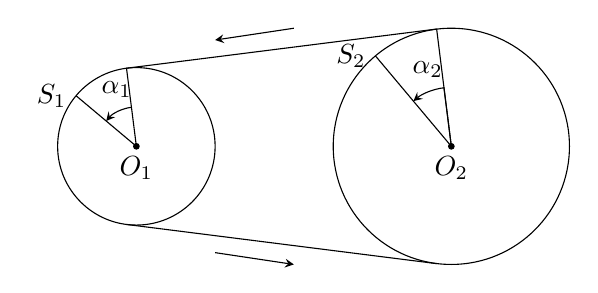
\begin{tikzpicture}[>=stealth]
\draw (0, 0) circle(1);
\draw (4, 0) circle(1.5);
\draw[fill=black] (0, 0) circle(1pt);
\draw[fill=black] (4, 0) circle(1pt);

\node[below] (O1) at (0, 0) {$O_1$};
\node[below] (O2) at (4, 0) {$O_2$};

%% 使用角度来找几何关系绘图(极坐标)
%% (a, b) --+ (c, d) : 表示把(a, b)看作坐标原点,或者说是后边邻近的坐标(c, d)是相对于(a, b)的相对坐标
\draw (140:1)node[left]{$S_1$} 
   -- (0, 0) 
   -- (97.2:1) 
   --+ (7. 2:3.97) 
   -- (4, 0) 
   --+ (130:1.5)node[left]{$S_2$};

%% 下边对称的直线只需符号取反即可。
\draw (-97.2:1) 
  --+ (-7. 2:3.97); 

%% 绘制圆弧arch命令
\draw[->] (97.2:0.5) arc (97.2:140:0.5); 
%% 下边由于O2不是原点,所以我们的想办法把它变为原点,这样就可以用arch方便的绘图
\draw[->] (4, 0) --+ (97.2:0.75) arc (97.2:130:0.75);
%% (4, 0) --+ (97.2:0.75): 这条线覆盖了原来的线

%% 直接使用坐标定位绘制剩余的标注
\node at (-0.25, 0.5)[above]{$\alpha_1$};
\node at (4-0.3, 0.75)[above]{$\alpha_2$};
\draw[<-] (1, 1.35) -- (2, 1.5);
\draw[->] (1, -1.35) -- (2, -1.5);
\end{tikzpicture}  
  
\end{center}